A regra \ref{reldeonticrole} tem os fundamentos teóricos na lógica deôntica e em modelos como \textit{MOISE+}. Assim sendo, todas as relações de obrigação implicam relações de permissão. O que essa regra determina consiste no fato de que se um agente $g_j$ é obrigado a trabalhar sob o objetivo $g_j$, então esse agente também tem a permissão de trabalhar sobre o objetivo $g_j$ 

\begin{eqnarray}\label{reldeonticrole}
	hasObligation(\rho_m,g_j) \to hasPermission(\rho_m,g_j), \nonumber \\
    \rho_m \in Role \wedge g_j \in Goal
\end{eqnarray}

As regras \ref{conditionViol}, \ref{relationViol}, e \ref{entityViol} são fundamentadas em \ref{normasdastani} onde o conceito do que pode ser feito é definido em termos das regras \textit{Count-as}. Essas regras determinam quais são os elementos que resultam em violação. Inspirando-se nesse tipo de estrutura é que os pesquisadores trataram de trabalhar as referidas regras. 

A complexidade de estudo é extramente ampla, e com certeza existe mais tipos de violações do que as três consideradas a seguir, contudo optou-se por estudar essas violações porque são essenciais para os objetivos deste estudo. Outro questionamento que pode surgir consiste no porque definir três tipos de violações? Isso reside no fato de que essas violações resultam em consequências diferentes, por conta disto em um primeiro momento os engenheiros do modelo decidiram tratá-las em estruturas diferentes. 

A explicação das regras será feita sempre analisando a semântica do predicado que é implicado em relação aos estudos pelos quais elas se fundamentam. Partindo desta premissa, o entendimento da relação \ref{conditionViol} só pode ser feito na ocorrência de uma  investigação sobre quais são os elementos que semanticamente correspondem ao predicado $conditionViol(ag_m,g_i,c_k)$. O primeiro ponto reside em verificar quais são as condições necessárias de $g_i$. Quem tem essa finalidade é o predicado $requiresCirc(g_i,c_k)$. Contudo, saber todas as condições não são o suficientes, pois a violação acontece na ausência de uma condição $c_k$ e isso deve ser verificado nesta relação de implicabilidade. Então se faz necessário considerar um predicado que analisa se $c_k$ está presente no ato da manutenção, e é com esse propósito que $isPresent(c_k)$ faz parte da relação. Contudo, as informações ficam desencontradas se $c_k$ não for uma instância de $Condition$, por isso é importante fazer essa análise também através do predicado $instanceOfCond(c_k)$. Esses são componentes essenciais, porém não são suficientes porque não consideram a condição do agente. Isso, pois afirmar sobre a ocorrência de uma violação de um agente sem considerar se ele esta efetivamente tentando alcançar um objetivo consiste em desconsiderar a semântica daquilo que está sendo implicado. Isso é resolvido por considerar o termo  $starts(ag_m,g_i)$. 

\begin{eqnarray}\label{conditionViol}\nonumber
	requiresCirc(g_i,c_k) \wedge \neg isPresent(c_k) \wedge instanceOfCond(c_k) \wedge starts(ag_m,g_i)  \to \\ \nonumber   
	conditionViol(ag_m,g_i,c_k) \nonumber \\  
    g_i \in Goal, c_k \in Condition, ag_m \in Agent
\end{eqnarray}

O propósito da regra \ref{conditionViol}, quando definido em termos de linguagem natural tem a finalidade de exprimir o seguinte: Se um agente tentar executar um determinado objetivo sem que haja todas as condições ambientes necessárias para isso, então esse agente comete uma violação de condição neste respectivo objetivo. 

A regra \ref{relationViol} define as condições que resultam em uma violação de relação. O predicado $relationViol(ag_m,g_i,r_k)$ considera que a violação se dá por um agente $ag_m$ em um objetivo $g_i$ na relação $r_k$. Portanto, para respeitar a semântica deste predicado se faz necessário considerar ao menos um termo que vincule o objetivo $g_i$ com a relação $r_k$. Para esse propósito é que se considera o termo $requiresCirc(g_i,circ_k)$ pois define quais são as circunstâncias que devem estar presentes para que o objetivo $g_i$ possa ser alcançado. Contudo, só isso não é o suficiente, pois se faz necessário analisar se $r_k$ está contido em $Relation$. Isso se deve ao fato de que o predicado $requiresCirc(g_i,circ_k)$ não permite saber se $circ_k$ está contido em $Relation$ ou se está contido em $Condition$. O predicado $instanceOfRel(r_k)$ resolve essa situação. Outro fator atrelado e importante para que o predicado $relationViol(ag_m,g_i,r_k)$ retorne verdade, reside em saber se o agente em sua tentativa de atingir $g_i$ não executa $r_k$ de forma apropriada. Por conta disso se faz necessário considerar o $isPresent(r_k)$. A semântica de $relationViol$ só é conservada em sua inteireza se a presença do agente também for analisada. Para esse propósito é que se verifica a necessidade do uso de $starts(ag_m,g_i)$ que deverá retornar se o agente está tentando alcançar o objetivo $g_i$.   

\begin{eqnarray}\label{relationViol}\nonumber
	requiresCirc(g_i,r_k)\wedge \neg isPresent(r_k) \wedge instanceOfRel(r_k) \wedge starts(ag_m,g_i) \to \nonumber \\
	relationViol(ag_m,g_i,r_k) \nonumber \\  
    g_i \in Goal, r_k \in Relation, ag_m \in Agent
\end{eqnarray}

Traduzindo a regra \ref{relationViol} para linguagem natural obtêm-se a seguinte expressão: Se um agente tentar alcançar um certo objetivo sem que todas as relações necessárias para isso estejam presentes (considerando as relações do domínio dele, tal como manuseio de uma ferramenta específica, e considerando as relações que são independentes dele), então esse agente comete uma violação de relação. 

A regra \ref{entityViol} tem o propósito de definir quais são as condições que resultam em uma violação de entidade. Como em outras situações, para cumprir com esse propósito é necessário que os fatores implicantes sejam correspondente com $entityViol(ag_m,g_i,e_k)$. Para cumprir com essa finalidade, se faz necessário considerar o predicado $requiresEntity(g_i,eg_n)$ (para avaliar as entidades que devem estar presentes a fim de cumprir com o objetivo $g_i$), $isPresent(e_k)$ (para verificar se a entidade $e_k$ está ou não, presente no momento da execução) e $starts(ag_m,g_i)$ (para avaliar se $ag_m$ começou a tentar alcançar o objetivo $g_i$). A semântica do predicado também considera o momento em que o agente está atuando sobre o objetivo $g_i$, por isso o predicado $starts(ag_m,g_i)$ também é posto na relação de implicabilidade.

\begin{eqnarray}\label{entityViol}\nonumber
	requiresEntity(g_i,eg_n) \wedge \neg isPresent(e_k) \wedge starts(ag_m,g_i) \to \nonumber \\ 
    entityViol(ag_m,g_i,e_k)  \nonumber \\  
    g_i \in Goal, e_k \in Entity, ag_m \in Agent
\end{eqnarray}

Em termos de linguagem natural, a regra \ref{entityViol} se apresenta da seguinte forma: Se um agente tentar alcançar um certo objetivo sem ter todas as entidades presentes para isso, então esse agente cometeu uma violação de entidade.

As regras \ref{consconditionViol} e \ref{consrelationViol} são inspiradas nos estudos presentes na seção \ref{normasdastani} onde as consequências de uma violação são definidas como sanções no que é denominado por $Sanction Rule$. A estrutura dessas regras, em \ref{normasdastani} e em \cite{dastaniframework} é dada como $violation \to ... $. Contudo, este estudo leva em consideração não apenas o termo que se refere a violação, mas também as circunstâncias que são consideradas juntas, que neste caso advêm do predicado $hasRisk$. Assim como em \ref{normasdastani}, o modelo deste estudo define que uma sanção corresponde a uma penalidade que o agente deve pagar. Na estrutura da problemática em análise, a penalidade ocorre pelo fato do agente sofrer fisicamente os efeitos dos seus erros. Esse comportamento é dado pelo predicado $negConseqFor(g_i,ag_m,risk_j,cs_m)$ cujo correspondente semântico define que o agente $ag_m$ sofre o evento associado em $risk_j$, no objetivo $g_i$ a consequência $cs_m$. Se os engenheiros deste modelo considerarem apenas $conditionViol(ag_m,g_i,c_k)$ para a relação \ref{consconditionViol} e $relationViol(ag_m,g_i,r_k)$, o correspondente semântico de $negConseqFor(g_i,ag_m,risk_j,cs_m)$ é desrespeitado, não especificando $risk_j,cs_m$. Contudo, isso é resolvido por levar em consideração o predicado $hasRisk(c_k,risk_j,cs_m)$ para \ref{consconditionViol} e o predicado $hasRisk(r_k,risk_j,cs_m)$ para \ref{consrelationViol}. 

\begin{eqnarray}\label{consconditionViol}\nonumber
	conditionViol(ag_m,g_i,c_k)  \wedge hasRisk(c_k,risk_j,cs_m) \to \nonumber \\ 
	negConseqFor(g_i,ag_m,risk_j,cs_m) \nonumber \\ 
    ag_m \in Agent, g_i \in Goal, c_k \in Condition, risk_k \in Risk, cs_m \in Consequence
\end{eqnarray}

Em termos de linguagem natural, a relação em \ref{consconditionViol} é definida da seguinte maneira: "Uma violação de condição de um determinado agente, em um dado objetivo ocasiona em uma consequência ruim a ele. Essa consequência ruim está associada ao risco da condição violada". 

\begin{eqnarray}\label{consrelationViol}\nonumber
	relationViol(ag_m,g_i,r_k) \wedge hasRisk(r_k,risk_j,cs_m) \to \\ 
	negConseqFor(g_i,ag_m,risk_j,cs_m) \nonumber \\ 
    ag_m \in Agent, g_i \in Goal, r_k \in Relation, risk_k \in Risk, cs_m \in Consequence 
\end{eqnarray}

A regra \ref{consrelationViol}, quando posta em linguagem natural é definida desta forma: "Uma violação de relação de um determinado agente, em um dado objetivo resulta em uma consequência ruim a ele. Essa consequência está atrelada ao risco da relação violada". 

Neste estudo o termo \textit{risco} deve ser analisado com muito cuidado. Isso, pois, dependendo do contexto, a complexidade deste termo é praticamente infinita e neste estudo a concepção deste termo se reduz a dois dos muitos possíveis usos. Neste modelo, risco é analisado como um evento que tem potencial de acontecer, contudo, nas relações de implicação um dos usos do termo risco advém de considerá-lo como evento que acontece apenas na ausência de uma dada condição ou de uma dada relação. Os pesquisadores optaram por essa tratativa ao estudar os conceitos presentes no referencial teórico em \ref{risksec} e ao analisar o caso de estudo (que será apresentado mais tarde). Com base nestes estudos, verificou-se que acidentes acontecem porque profissionais tentam executar uma certa atividade sem ter as condições apropriadas para isso e é à essa circunstância sobre o qual o risco está associado (em \cite{safety}, isso é explicado visando a melhoria da eficiência e da produção). Por exemplo, para poder navegar em alto mar a fim de poder pescar, um barco pesqueiro deve ter a sua disposição uma determinada condição climática. Se a tripulação decidir por navegar sem a presença da condição climática apropriada, então o barco está submetido ao risco de naufragar sob as consequências de morte da tripulação inteira. Portanto é com essa semântica que as relações de implicação \ref{consconditionViol} e \ref{consrelationViol} empregam o conceito de risco. 

Obviamente, existe a possibilidade do barco poder desbravar um mar sem as apropriadas condições e voltar para a terra a salvo. Contudo, considerar situações assim, apesar de serem interessantes, levam a um aprofundamento da complexidade deste modelo. Não que isso seja uma justificativa coerente para não se fazer isso, contudo - neste estudo o interesse reside em uma primeira versão que torne possível a modelagem de condições assim por meio de um vocabulário mais específico. Assim sendo, os pesquisadores decidiram por simplificar essa situação e considerar que toda a ação tomada por um agente sem que as condições necessárias estejam presentes, ou as relações apropriadas sejam feitas, resultam em penalidades associadas ao risco da ausência desses elementos.  

Dentro do que condiz ao conceito de sanção que é tratado neste estudo, apenas as regras \ref{consconditionViol} e \ref{consrelationViol} são sanções. Isso se deve ao fato de que essas regras consideram que o equívoco do agente, gerou penalidades a ele mesmo. Apesar de levar em consideração predicados associados a violação, as demais regras não são consideradas como regras de sanção porque elas apresentam uma condição onde o comportamento inapropriado de um agente A, resulta em consequências ruins a outros agentes. Como o erro do agente A não recai sobre si, é um inequívoco, dentro do escopo deste estudo, afirmar que ele sofreu uma sanção por conta disto. 


A regra \ref{entityViolaffect} é usada com o propósito de demonstrar que uma dada violação em uma certa relação afeta outras relações. Isso, pois muitas vezes o ato de não executar uma determinada relação não gera consequências imediatas no instante a ser considerado, contudo essas consequências se manifestam em relações futuras. Não somente isso, mas a regra \ref{entityViolaffect} também considera um dado componente de aleatoriedade que está atrelado com este tipo de raciocínio. O predicado $possOfNegConseqFor(r_n)$ semanticamente corresponde que existe a possibilidade de acontecer algo errado associado ao relacionamento $r_n$. O sentido deste termo é correspondido quando se verifica os elementos que causam este tipo de condição - que no caso desta regra isso envolve a ocorrência de uma violação em $r_k$, sendo que esse relacionamento afeta $r_n$.

\begin{eqnarray}\label{entityViolaffect}
	relationViol(ag_m,g_i,r_k) \wedge affectsRels(r_k,r_n) \nonumber \\
    \to possOfNegConseqFor(r_n)  \nonumber \\
    ag_m \in Agent, g_i \in Goal, r_k,r_n \in Relation, 
\end{eqnarray}

O entendimento desta regra pode ser feito ao considerar um exemplo que já foi mencionado neste texto ao apresentar o correspondente do predicado \textit{possOfNegConseqFor} e o predicado \textit{affectsRels}, onde um eletricista usa um bastão isolante para acessar um dado barramento. Naquela parte do texto o problema é modelado por meio de duas relações; $relBastaoMedidor$ (que define a relação que deve ser feita entre o bastão isolante com um aparelho medidor de correte de fuga) e $relBastaoBarramento$ (que consiste na relação entre o bastão com o barramento elétrico do quadro de energia). Tendo em vista que a ausência de uma medida em $g_{medida}$ afeta a possibilidade de ocorrer algum evento grave em $relBastaoBarramento$, é dado - para esse caso - como verdade o seguinte predicado $affectsRels(relBastaoMedidor, relBastaoBarramento)$. Assim sendo, em um cenário em que ocorre a violação de relação em $g_{medida}$, o seguinte raciocínio pode ser feito: $relationViol(eletricista_{medidor},g_{medida},relBastaoMedidor) \wedge affect(relBastaoMedidor, relBastaoBarramento) $ \\ $\to  possOfNegConseqFor(relBastaoBarramento)$.   

A regra \ref{entityViolaffect} demonstra como um agente pode ser submetido a consequências ruins sem necessariamente ser culpado por isso. Contudo, essa regra denota apenas possibilidade, não demonstrando o que acontece efetivamente quando o agente é submetido ao lado não favorável da possibilidade. Essa situação está atrelada a \ref{paybutiamnotguilty}. Para lidar com as situações onde um agente é submetido a condições ruins, fez-se o uso do predicado $possOfNegConseqFor(g_i,ag_m,risk_j,cs_m) $. Entretanto, diferente das regras \ref{consconditionViol}, \ref{consrelationViol}, essas consequências negativas tem seus correspondentes semânticos em outros predicados. O predicado $possOfNegConseqFor(r_k)$ é invocado com o propósito demonstrar que $r_k$ apresenta a possibilidade da ocorrência de um evento ruim mesmo que o agente que esteja executando essa relação não faça nada de errado. Contudo, esse predicado só denota a possibilidade. Para que o sentido semântico de que a possibilidade de um evento ruim realmente acontece foi considerado o uso do predicado $happensNegConseqFor(r_k)$. Para o contexto desta regra, a semântica deste predicado exibe o seguinte significado: "O evento ruim associado a essa relação realmente aconteceu". Nesta situação que se faz necessário adotar a outra concepção associada ao termo risco que é adotado a este modelo. Nesta regra, esse termo é adotado como um evento em potencial devido a incerteza associada ao evento. 

Para compreender melhor essa situação é possível voltar ao exemplo do eletricista-bastão isolante-quadro de energia. Como já citado anteriormente o fato do agente medidor não executar sua atividade gera uma incerteza sobre a condição do isolamento do bastão. Se a medida for executada com sucesso (partido do pressuposto de que o medidor está em condições apropriadas de funcionamento), a condição do bastão é revelada eliminando qualquer incerteza a respeito disto. Contudo, como está sendo considerado um cenário em que isso não foi feito, a não execução de $relBastaoMedidor$ resultou no surgimento do risco $eletrocutado$ com uma consequência de morte. Esse risco é definido como um potencial evento até que o eletricista de acesso ao barramento faz uso da ferramenta. Por conta disto, se usa o predicado $hasRisk(r_k,risk_j,cs_m)$. Tendo em vista que isso se dá por uma relação que está atrelada a um objetivo, se faz necessário considerar $requiresCirc(g_i,r_k) \wedge (r_k \in rg_n) $ e  $instanceOfRel(r_k)$ . Para verificar a ação do agente nesta situação, o predicado $starts(ag_m,g_i)$ também deve compor a regra.


\begin{eqnarray}\label{paybutiamnotguilty}
	possOfNegConseqFor(r_k) \wedge  happensNegConseqFor(r_k) \wedge requiresCirc(g_i,r_k) \nonumber \\ 
	\wedge instanceOfRel(r_k) \wedge hasRisk(r_k,risk_j,cs_m) \wedge starts(ag_m,g_i) \nonumber \\ 
	\to negConseqFor(g_i,ag_m,risk_j,cs_m) \nonumber \\ 
    r_k \in Relation, g_i \in Goal, risk_k \in Risk, cs_m \in Consequence
\end{eqnarray}

O exemplo em voga pode ser implementado nesta regra da seguinte forma: 

\begin{eqnarray}\nonumber
   possOfNegConseqFor(relBastaoBarramento) \nonumber \\
    \wedge happensNegConseqFor(relBastaoBarramento) \nonumber \\ 
    \wedge requiresCirc(g_{acessoBarramento},relBastaoBarramento) \nonumber \\  
    \wedge instanceOfRel(relBastaoBarramento) \nonumber \\ 
    \wedge hasRisk(relBastaoBarramento,eletrocutado,morte) \nonumber \\  
    \wedge starts(eletricista_{executor},g_{acessoBarramento}) \nonumber \\ 
    \to negConseqFor(g_{acessoBarramento},eletricistaExecutor,eletrocutado,morte) \\ \nonumber
\end{eqnarray}

O exemplo se traduz na situação em que um bastão apresenta uma possibilidade de estar com o seu isolamento comprometido e isso resulta em um risco de eletrocutar o profissional que o usa resultando na morte dele. Portanto, no momento em que a ferramenta é usada o eletricista morre eletrocutado, por que esse bastão pertencia as ferramentas cujo isolamento estava deteriorado. 

A violação de entidade, dada pela regra \ref{consvioent}, diferente das demais, resulta apenas no encerramento da atividade referente ao objetivo onde o método foi invocado. Os engenheiros desse modelo definiram essa regra partindo do pressuposto que a ausência de uma ferramenta, profissional, peça de substituição ou máquina simplesmente gera o impedimento do prosseguimento das atividades. Voltando ao exemplo do eletricista, se o profissional não tiver o bastão isolante para executar a ação, ele simplesmente não consegue dar prosseguimento ao objetivo fazendo com que o procedimento seja encerrado naquele exato instante. 

\begin{eqnarray}\label{consvioent}
	entityViol(ag_m,g_i,e_k) \to stopped(g_i) \nonumber \\  
    ag_m \in Agent, g_i \in Goal, e_k \in Entity \\ \nonumber
\end{eqnarray}

Em termos de linguagem natural, a regra \ref{consvioent} é definida da seguinte forma: Se acontecer uma violação de entidades, então o procedimento é encerrado no objetivo onde aconteceu. 

A regra \ref{badcons} advém do pressuposto de que na ocorrência de uma calamidade onde um profissional sai extremamente ferido ou morto (ocorrência do acidente), os demais envolvidos na manutenção não continuam por executar os procedimentos. 
 
 \begin{eqnarray}\label{badcons}
	negConseqFor(g_k,ag_m,risk_j,cs_m) \to stopped(g_k) \nonumber \\ 
    g_k \in Goal, risk_j \in Risk, cs_m \in Consequence
\end{eqnarray}

Essa regra, no escopo da linguagem natural, pode ser lida desta forma: Se acontecer um evento ruim em que um profissional sai morto ou gravemente ferido, então a manutenção é encerrada no objetivo onde a fatalidade aconteceu. Não há como afirmar que as regras  \ref{consvioent} e \ref{badcons} se aplicam para todo tipo de situação em qualquer procedimento. Operações militares, por exemplo, não se enquadram em situações assim. Isso, pois a morte de um soldado ferido não impede que o resto do batalhão continue em conflito. Contudo, os pesquisadores deste estudo entendem que o pressuposto dessas duas regras englobam diversos cenários que implica no interesse deste estudo, tais como; cenário industrial, subestação, usinas de produção de energia, certas atividades hospitalares e entre outras da mesma natureza.  

A regra estabelecida pela figura \ref{wenStop} define o critério para quando um dado objetivo é considerado como atingido. Isso ocorre quando todos os agentes $ag_n | n = i ... j$ que são obrigados a atingir um certo objetivo $ g_k $ fazem isso sem a ocorrência e uma interrupção $stopped(g_k,ag_n)$. A expressão \ref{wenStop} retrata isso. Diferente das outras regras, os pesquisadores preferiram especificar essa expressão como um algoritmo que avalia se um determinado objetivo foi interrompido agente por agente através de um \textit(foreach) sobre $agentArray$ (um $array$ que trás todos os agentes que tentaram alcançar o objetivo $goal$). Se o teste dado por $if(stopped(goa,agent))$ retorna verdade para pelo menos um dos agentes, então a função $ifNotStopped(agentArray,goal)$ retorna falso. Se essa situação não acontecer para todos os agentes carregados em $agentArray$, então o algoritmo determina um segundo teste, que é dado pela função $allAgentObligate(agentArray,goal)$. Essa função verifica se todos os agentes que são obrigados a alcançar o objetivo $goal$ estão contidos em $agentArray$. No contexto desse algoritmo, se a função $allAgentObligate(agentArray,goal)$ retorna falso, então $ifNotStopped$ também retorna falso, caso contrário $ifNotStopped$ retorna verdade. Se a função $ifNotStopped(agentArray,goal)$ retorna verdade, então o predicado $reached(goal)$ é verdade também.

\begin{figure}[H]
  \centering
  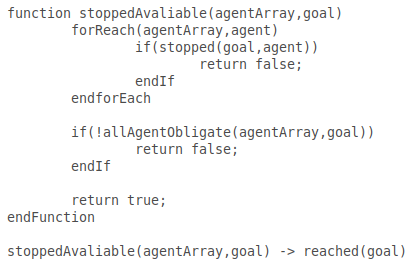
\includegraphics[width=0.6\linewidth]{figure/algfigthree.png} 
  \caption{Condição para definir se um dado objetivo foi atingido ou não} \label{wenStop}  
\end{figure}

Na linguagem natural essa expressão fica da seguinte forma: Se todos os agentes que têm permissão para alcançar um dado objetivo fizeram sem que esse tenha sido interrompido e considerando que um subgrupo deles é constituído por agentes que são obrigados a isso, então o objetivo é dado como alcançado.

A regra \ref{rolenextgoal} apresenta a condição adequada para quando um agente está habilitado para atingir novos objetivos. Para isso, ele deve possuir um papel onde existe uma permissão para que ele possa atingir o próximo objetivo. Isso é traduzido por $ adoptsRole(ag_n,\rho_m) \wedge hasPermission(\rho_m,g_j) $. Não apenas isso, mas o objetivo atual do agente deve ter sido atingido $ reached(g_i) $ e o objetivo em interesse deve estar associado como predicado $nextGoal(g_i,g_j)$. O termo $enabledToStart(ag_i,g_j)$ corresponde semanticamente apenas que o agente está habilitado a buscar novos objetivos mas não significa que isso implicará em $starts(ag_i,g_j)$ pois o que decide esses processos de transição consiste em aspectos que não correspondem a esse modelo. Essa dinâmica é discutida mais tarde na seção de \textit{Predicados de Controle}.

\begin{eqnarray}\label{rolenextgoal}
	adoptsRole(ag_n,\rho_m) \wedge hasPermission(\rho_m,g_j) \wedge nextGoal(g_i,g_j) \wedge reached(g_i) \nonumber \\
	\to enabledToStart(ag_i,g_j) \nonumber \\
    ag_i, ag_n \in Agent, \rho_m \in Role, g_j \in Goal, g_i \in Goal
\end{eqnarray}

Em linguagem natural, a regra \ref{rolenextgoal} exibe o seguinte: "Se um agente que alcançou um objetivo atual tem um papel que lhe dá permissão para buscar o próximo objetivo, então esse agente está habilitado para fazer isso"

A regra \ref{rolelastgoal} apresenta a condição de parada do agente em relação ao seu papel. Isso, pois se o agente, que tem um determinado papel, cumpriu com todos os objetivos designados a ele, então ele deve encerrar sua operação. A verificação do papel é dado por $adoptsRole(ag_n,\rho_m) \wedge hasPermission(\rho_m,g_i)$, a análise semântica sobre o último objetivo associado a um certo papel é dado por $lastGoal(g_i,\rho_m)$ e a verificação se aquele último objetivo foi atingido é dado por $reached(g_i)$. 

\begin{eqnarray}\label{rolelastgoal}
	adoptsRole(ag_n,\rho_m) \wedge hasPermission(\rho_m,g_i) \wedge lastGoal(g_i,\rho_m) \wedge reached(g_i) \nonumber \\
	\to stopped(g_i) \nonumber \\
    ag_n \in Agent, \rho_m \in Role, g_i \in Goal
\end{eqnarray}

Portanto, a regra \ref{rolelastgoal} em linguagem natural é definida da seguinte maneira; Se um agente cumpriu com todos os objetivos associados a permissão do papel dele, então esse agente deve encerrar suas atividades (em relação a esse papel). 
